\section{Mesure des temps de relaxation}
\subsection{Mesure de $T_1$}
La mesure du temps de relaxation longitudinale nécessite 
\begin{itemize}
\item d'amener la composante $\aimzs$ de l'aimantation $\aimvec$ hors de
sa valeur d'équilibre $\aimzerozs$
\item de laisser évoluer $\aimvec$ pendant des temps $\tau$ convenablement choisis,
\item de convertir l'aimantation longitudinale "relaxée" en aimantation transversale
détectable
\item d'enregistrer les FID pour les différentes valeurs de $\tau$
\item d'étudier la variation de l'intensité des résonances en fonction de $\tau$
pour déduire la valeur de $T_1$.
\end{itemize}
La première étape est réalisable soit par saturation de l'aimantation
($\aimvec = \zerovec$, section \ref{sec:eqnbloch}), soit par inversion
au moyen d'une impulsion d'angle $\pi$.
La seconde solution est celle qui procure le plus grand écart possible 
entre $\aimzs$ et $\aimzerozs$ et qui est la plus simple à mettre en {\oe}uvre ;
c'est celle qui est généralement retenue.
La séquence impulsionnelle correspondante est décrite dans la figure \ref{fig:mesuretun}.

\begin{figure}[hbt]
\begin{center}
\begin{pspicture}(0,0)(7,3)
% sequence I
\rput(1,1.5){
\psline(0,0)(6,0)
\rput(-0.5,0){RF($I$)}
\psline[linewidth=4mm]{-}(1,0)(1,1)
\rput(1,1.2){$\phi_1$}
\psline[linewidth=2mm]{-}(4,0)(4,1)
\rput(4,1.2){$\phi_2$}
\rput(4.1,0){
\pscurve(0,0.5)(0.5,0.25)(1.5,0)
\pscurve(0,-0.5)(0.5,-0.25)(1.5,0)
\psline(0,0.5)(0,-0.5)
}
\rput(5,0.5){$\phi_R$}
}
% time marks
\rput(1,0.5){
\psline{->}(0,0)(6,0)
\psline[linewidth=0.25mm,linestyle=dashed]{-}(0.8,0.8)(0.8,-0.2)
\rput(0.8,-0.4){0}
\psline[linewidth=0.25mm,linestyle=dashed]{-}(1.2,0.8)(1.2,-0.2)
\rput(1.2,-0.4){1}
\rput(2.5,0.5){$\tau$}
\psline[linewidth=0.25mm,linestyle=dashed]{-}(3.9,0.8)(3.9,-0.2)
\rput(3.8,-0.4){2}
\psline[linewidth=0.25mm,linestyle=dashed]{-}(4.1,0.8)(4.1,-0.2)
\rput(4.2,-0.4){3}
\psline[linewidth=0.25mm,linestyle=dashed]{-}(3,0.8)(3,-0.2)
\rput(3,-0.4){$t$}
}
\end{pspicture}
\caption{\label{fig:mesuretun}
Mesure de $T_1$}
\end{center}
\end{figure}

Quelle que soit la phase $\phi_1$ de la première impulsion, 
l'état initial $\sigma_0$ d'un noyau $I$ est transformée en $\sigma_1 = -I_z$.
D'une manière plus générale, à l'instant 1, $\aimz = -\alpha\aimzerozs$ où
$\alpha = 1$ pour une inversion parfaite et $\alpha = 0$ 
pour la saturation totale de $\aimvec$.
En écrivant $m(t) = \aimzs(t) - \aimzerozs$ (ici $t=0$ correspond à l'instant 1),
l'équation \ref{eqn:t1} devient
\begin{equation}
\derivt{m(t)} = -\frac{m(t)}{T_1}
\end{equation}
dont la solution est
\begin{equation}
m(t) = m(0) \exp\left(-\frac{t}{T_1}\right)
\end{equation}
Sachant que $m(0) = -(1+\alpha)\aimzerozs$,
\begin{equation}
\aimzs(\tau) = \aimzerozs\left(1-(1+\alpha)\exp\left(-\frac{\tau}{T_1}\right)\right)
\end{equation}

L'aimantation longitudinale à l'instant 2 est convertie
en aimantation transversale détectable à partir de l'instant 3, qui fournit un signal
proportionnel à $\aimzs(\tau)$.
L'intensité $I(\tau)$ du pic spectral issu du noyau $I$ est alors
\begin{equation}
\label{eqn:loit1}
I(\tau) = I(\infty)\left(1-(1+\alpha)\exp\left(-\frac{\tau}{T_1}\right)\right)
\end{equation}
puisque le signal maximal est obtenu lorsque l'aimantation a pu "relaxer"
pendant un temps plusieurs fois supérieur à $T_1$.
Plus précisément, si $\alpha = 1$ alors $I(5T_1)$ = 0.987, ce qui peut être considéré
comme égal 1 à 1,3 \% près et satisfaisant en fonction des autres sources d'erreur.
L'extraction de la valeur de $T_1$ à partir des intensités mesurées pour un ensemble
de valeurs de $\tau$ est du ressort des techniques d'ajustement non linéaire,
sauf si on considère comme connue la valeur de $I(\infty)$. Alors,
\begin{equation}
\log(1+\alpha) - \frac{\tau}{T_1} = \log\left(1-\frac{I(\tau)}{I(\infty)}\right)
\end{equation}
La représentation graphique de la fonction $f(\tau)$ définie par
\begin{equation}
f(\tau) = \log\left(1-\frac{I(\tau)}{I(\infty)}\right)
\end{equation}
est une droite de pente $-1/T_1$ et d'abscisse à l'origine $\log(1+\alpha)$.

L'inversion incomplète de l'aimantation peut avoir pour origine
soit une mauvaise calibration de l'impulsion, soit l'effet d'offset (ou les deux).
Les figures \ref{fig:offres}, et à plus forte raison, \ref{fig:veryoffres}
montrent qu'une inversion parfaite n'est possible que pour un noyau
en résonance ou très proche de la résonance.
L'inversion incomplète peut être combattue par l'utilisation
d'une impulsion composite.

L'impulsion composite d'inversion la plus simple qu'il soit possible d'imaginer
est dérivée de l'expression de l'hamiltonien réduit pour un système à un spin
établie à la section \ref{sec:echo1spin} et qui peut se résumer par
\begin{equation}
\label{eqn:rot1spin}
\flham{\alpha I_z}\quad\flham{\pi I_x}\quad\flham{\alpha I_z}
\iff
\flham{\pi I_x}
\end{equation}
puisque l'hamiltonien réduit, sans ce cas, est nul.
La permutation circulaire des axes O$X$, O$Y$ et O$Z$
($Z \rightarrow X$, $X \rightarrow Y$ et $Y \rightarrow Z$) laisse 
formellement l'équivalence des rotations \ref{eqn:rot1spin} inchangée :
\begin{equation}
\label{eqn:incompv}
\flham{\alpha I_x}\quad\flham{\pi I_y}\quad\flham{\alpha I_x}
\iff
\flham{\pi I_y}
\end{equation}

La séquence d'impulsions $\alpha_x$ --- $2\alpha_y$ --- $\alpha_x$ est donc
équivalente à une impulsion $\pi_y$ lorsque $\alpha = \pi/2$.
La propriété intéressante de cette séquence est qu'elle assure une
meilleure inversion que l'impulsion $2\alpha_y$ (ou $2\alpha_x$, de manière équivalente)
lorsque $\alpha$ est voisin de $\pi/2$.
Cela est clairement visible sur la figure \ref{fig:invcomp}.
A droite, l'impulsion centrale amène l'aimantation
du dessus du plan transversal vers le dessous, dans une position
quasiment symétrique, et rend ainsi possible une meilleure inversion qu'à gauche.

\begin{figure}[hbt]
\begin{center}
$a$
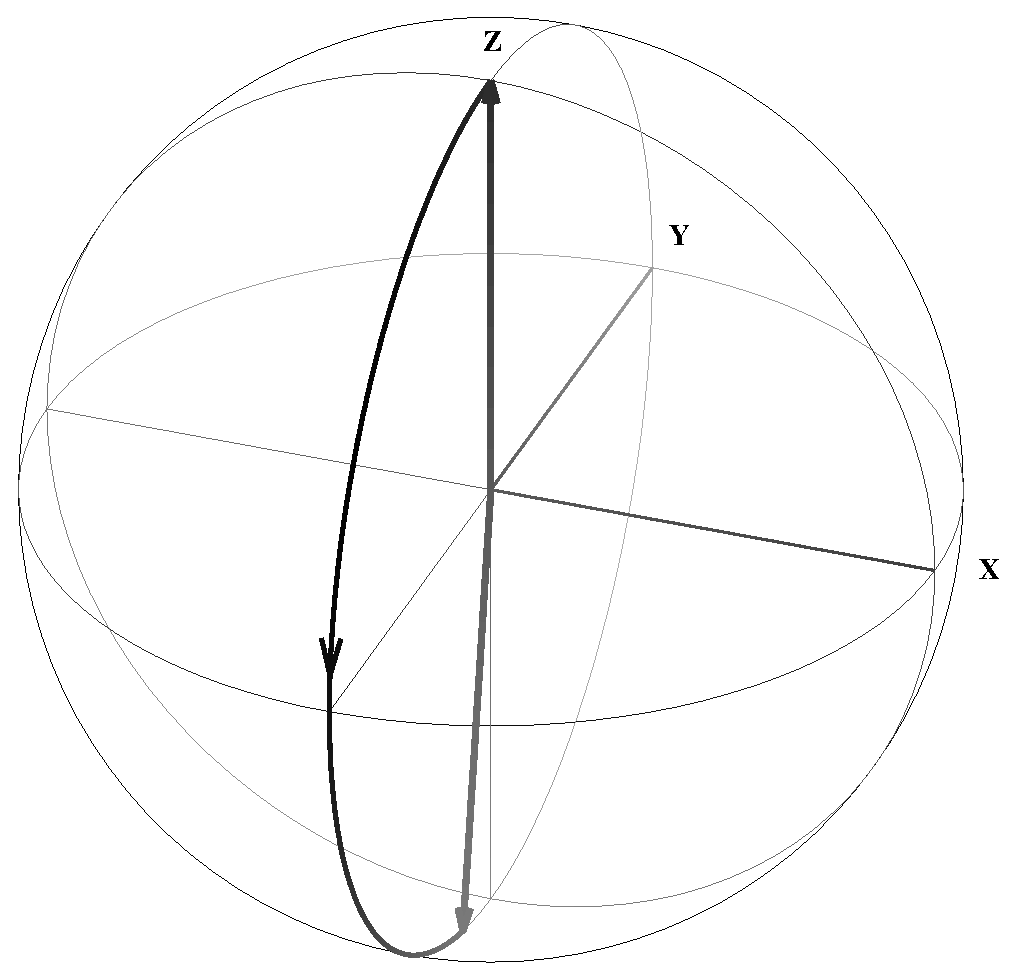
\epsfig{file=invcomp0.eps,width=2.5in}
\hspace{1em}
$b$
\epsfig{file=invcomp1.eps,width=2.5in}
\end{center}
\caption[Inversion composite]{Effet d'une erreur de calibration
sur l'inversion de l'aimantation d'équilibre.
A gauche l'inversion est effectuée par une impulsion $170^{\circ}_x$.
et à droite par la séquence $85^{\circ}_x$ --- $170^{\circ}_y$ --- $85^{\circ}_x$.}
\label{fig:invcomp}
\end{figure}

Une méthode rapide de mesure de $T_1$ consiste à utiliser la séquence de la figure
\ref{fig:mesuretun} et à rechercher expérimentalement la valeur $\tau_0$ de $\tau$
telle que $I(\tau_0) = 0$.
L'équation \ref{eqn:loit1} avec $\alpha = 1$ donne alors
\begin{equation}
\tau_0 = T_1 \log(2).
\end{equation}
ce qui permet d'évaluer $T_1$.

\subsection{mesure de $T_2$}
La démarche adoptée ici est la même que celle qui précède, à savoir une
"préparation" de l'aimantation qui révèle la grandeur à mesurer,
suivie de l'enregistrement du spectre proprement dit.
Pour mesurer $T_2$, il faut donc laisser évoluer l'aimantation transversale
pendant un temps $\tau$ puis détecter l'évolution libre de $\aimvec$.
Pendant le temps $\tau$, $\aimvec$ évolue sous l'action de l'offset $\omsi$
du noyau $I$ étudié, offset qui dépend de la localisation du noyau $I$
dans l'échantillon si $\bzeroz$ est inhomogène.
On mesurerait alors plutôt $T_2^*$ que $T_2$ (voir figure \ref{fig:isochrom}).
Une séquence d'écho de spin de durée $\tau$ permet de rendre l'évolution
de $\aimvec$ indépendante de $\omsi$.
Le cas où $I$ est scalairement couplé à un autre noyau de même type
sera traité en détail dans le cadre de la spectroscopie 2D $J$-résolue (---).
L'écho de spin est alors incapable de compenser l'action de l'opérateur 
de couplage qui subsiste dans l'hamiltonien réduit 
(equation \ref{eqn:hredis}) et qui introduit
une distorsion de phase.
L'analyse des données expérimentales devient alors
beaucoup plus difficile.
Toutefois, le $T_2$ d'un noyau couplé peut être mesuré
à condition que $J \tau \ll 1$ pour toutes les valeurs de $\tau$ utilisées.

En pratique, la préparation de l'aimantation consiste à faire subir
1, 2, 3, ..., $n$ séquences d'écho de spin de durées identiques $\tau_1$.
Les durées $\tau$ d'évolution de l'aimantation transversale sont alors
$\tau_1$, $2\tau_1$, $3\tau_1$, ..., $\tau_n = n\tau_1$ (Figure \ref{fig:mesuret2}).

\begin{figure}[hbt]
\begin{center}
\begin{pspicture}(0,0)(7,2)
% sequence I
\rput(0,-0.5){
\rput(1,1){
\psline(0,0)(6,0)
\rput(-0.5,0){RF($I$)}
\psline[linewidth=2mm]{-}(1,0)(1,1)
\rput(0.8,1.2){$\phi_1$}
\psline[linewidth=4mm]{-}(2.5,0)(2.5,1)
\rput(2.5,1.2){$\phi_2$}
\rput(3.9,0){
\pscurve(0,0.5)(0.5,0.25)(1.5,0)
\pscurve(0,-0.5)(0.5,-0.25)(1.5,0)
\psline(0,0.5)(0,-0.5)
}
\rput(5,0.5){$\phi_R$}
}
\rput(1,0.5){
\psline{->}(2,0)(1.1,0)
\psline{->}(3,0)(3.9,0)
\rput(2.5,0){$\tau_1$}
}
\rput(2.1,0.75){
\psline(0.25,0)(0,0)(0,1.5)(0.25,1.5)
}
\rput(4.9,0.75){
\psline(-0.25,0)(0,0)(0,1.5)(-0.25,1.5)
\rput(0.7,1.6){$n$ fois}
}
}
\end{pspicture}
\caption{\label{fig:mesuret2}
Mesure de $T_2$}
\end{center}
\end{figure}
A ce niveau de l'analyse, l'intensité du signal enregistré après
un temps d'écho $\tau_n$ est donnée par 
\begin{equation}
I(\tau_n) = \pm I(0) \exp\left(-\frac{\tau_n}{T_2}\right)
\end{equation}
Le signe de $I(\tau_n)$ dépend de la relation entre $\phi_1$ et $\phi_2$
et de la parité de $n$.
En effet, si $\phi_2 = \phi_1 \pm \pi/2$ (séquence 1), alors l'opérateur qui décrit
l'état du système juste après la première impulsion commute avec
l'opérateur associé aux impulsions de refocalisation.
Le signe de $I(\tau_n)$ est alors invariable.
Si $\phi_2 - \phi_1$ vaut 0 ou $\pi$ (séquence 2), les opérateurs en question ne commutent
pas et chaque écho multiplie $I(\tau_n)$ par $-1$.
La supériorité de la séquence 1 sur la séquence 2
est manifeste si on considère l'impact des imperfections
des impulsions de refocalisation sur le signal,
imperfections dues à une mauvaise calibration de $\buns$
(ou a son homogénéité dans l'échantillon) ainsi qu'à l'effet d'offset.
Il faut pour s'en rendre compte étudier les évènements qui se déroulent
pendant deux échos successifs (Figures \ref{fig:doublecho} et \ref{fig:cpmgcalib}).

\begin{figure}[hbt]
\begin{center}
\begin{pspicture}(0,0)(7,2)
\psline(0,0.5)(7,0.5)
\psline[linestyle=dashed,dash=2pt 2pt](0.5,0.3)(0.5,2)
\rput(0.5,0){A}
\rput(3.5,0){D}
\psline[linestyle=dashed,dash=2pt 2pt](3.5,0.3)(3.5,2)
\rput(6.5,0){G}
\psline[linestyle=dashed,dash=2pt 2pt](6.5,0.3)(6.5,2)
\rput(0.5,0.5){
\psline[linewidth=4mm]{-}(1.5,0)(1.5,1)
\psline{->}(1,1.5)(0,1.5)
\psline{->}(2,1.5)(3,1.5)
\rput(1.5,1.5){$\tau$}
\rput(1.3,-0.5){B}
\rput(1.7,-0.5){C}
}
\rput(3.5,0.5){
\psline[linewidth=4mm]{-}(1.5,0)(1.5,1)
\psline{->}(1,1.5)(0,1.5)
\psline{->}(2,1.5)(3,1.5)
\rput(1.5,1.5){$\tau$}
\rput(1.3,-0.5){E}
\rput(1.7,-0.5){F}
}
\end{pspicture}
\caption[Double écho de spin]{Double écho de spin. Les instants
marqués A à G font référence à la figure \ref{fig:cpmgcalib}.}
\label{fig:doublecho}
\end{center}
\end{figure}

Pendant les périodes de précession libre (A$\rightarrow$B, C$\rightarrow$D,
D$\rightarrow$E et F$\rightarrow$G), l'aimantation tourne d'un même angle 
autour de l'axe $OZ$ (dans cet exemple, il vaut 45\degres) et l'angle des
impulsions de refocalisation n'est pas $\pi$ (ici, il vaut 160\degres).
L'aimantation à l'instant D, dans la figure de gauche (séquence 1), 
est située au dessus du plan transversal au lieu d'être dessus,
comme ce serait le cas si l'impulsion était parfaite.
Cette erreur est compensée par le deuxième écho et l'aimantation en G
n'est que faiblement différente de celle à l'instant initial A.
La figure de droite montre que si $\phi_2 = \phi_1$ (séquence 2), l'aimantation
en D arrive en dessous du plan transversal et
s'en retrouve deux fois plus éloigné en G à l'issue du second écho.
L'effet des erreurs de calibration est alors cumulatif.

\begin{figure}[hbt]
\begin{center}
$a$
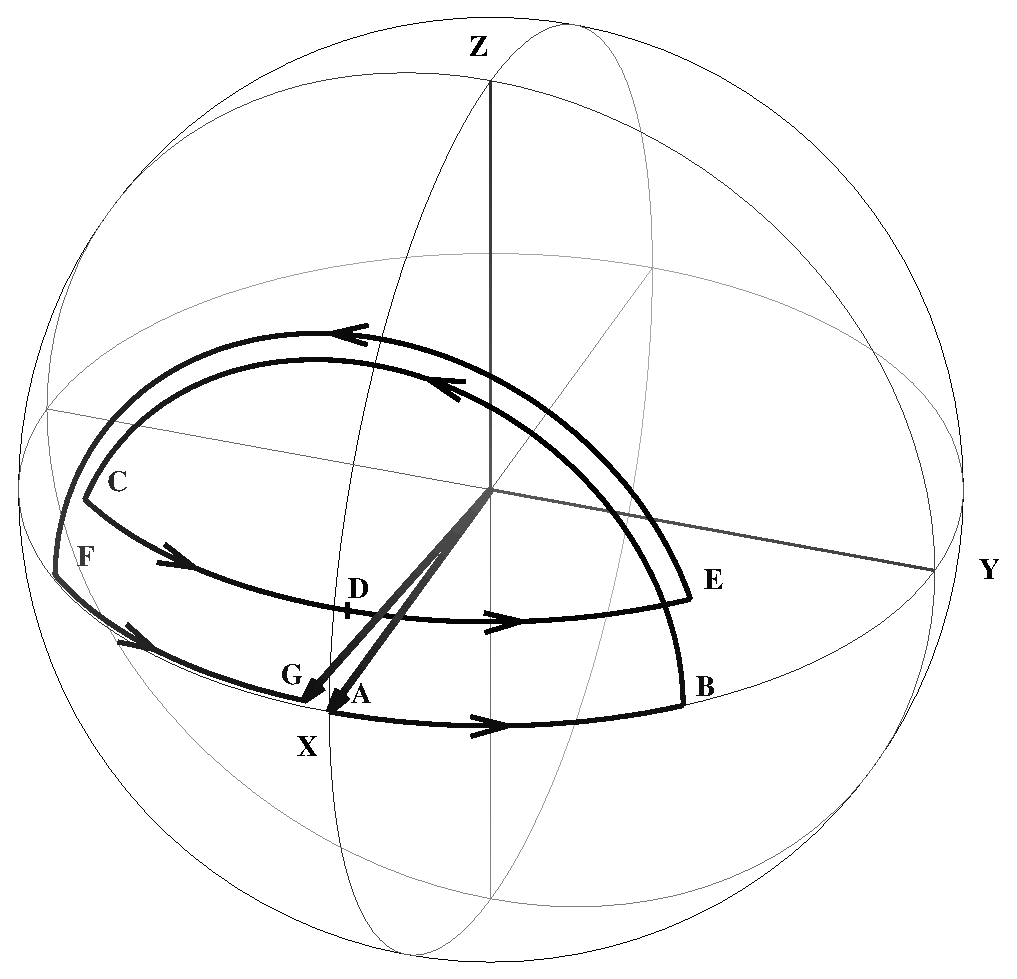
\epsfig{file=cpmgcalib0.eps,width=2.5in}
\hspace{1em}
$b$
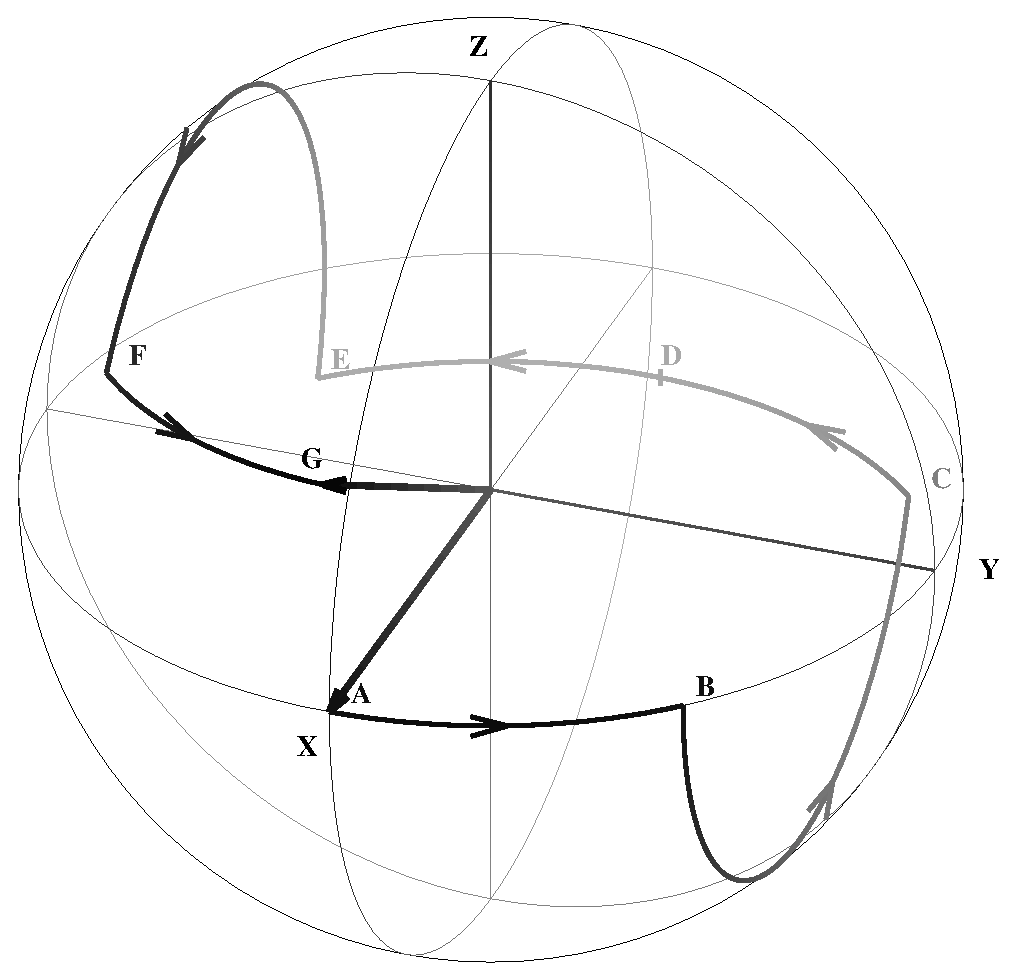
\epsfig{file=cpmgcalib1.eps,width=2.5in}
\end{center}
\caption[Séquence CPMG]{Effet d'une erreur de calibration sur l'évolution de
l'aimantation au cours d'un double écho de spin.
A gauche $\phi_2 - \phi_1 = \pi/2$ (Séquence 1, ou CPMG) 
et à droite $\phi_1 = \phi_2$ (Séquence 2, ou CP).}
\label{fig:cpmgcalib}
\end{figure}

La séquence 2 est aussi appelée séquence de Carr--Purcell.
Elle a été améliorée
par le déphasage de $\pi/2$ des impulsions de refocalisation par rapport à
l'impulsion d'excitation pour aboutir à séquence de Carr--Purcell--Meiboom--Gill
(CPMG).
L'enregistrement des signaux qu'elle produit lorsque $n$ est pair minimise
les erreurs sur la mesure de $T_2$.

La valeur de $T_2$ est obtenue à partir de la représentation graphique
de la fonction $f(\tau_n)$ définie par
\begin{equation}
f(\tau_n) = \log\left(\frac{I(\tau_n)}{I(0)}\right) = -\frac{\tau_n}{T_2}
\end{equation}
La fonction $f(\tau_n)$ est linéaire et sa pente est $-1/T_2$.

La non--équivalence d'un écho de durée totale $n\tau_1$ et de $n$ échos
de durée $\tau_1$ n'apparaît que lorsqu'on considère le mouvement
brownien des molécules au sein de l'échantillon liquide et l'existence
du gradient $\sgvec$ de $\bzerozs$, constant dans le temps, et dû au réglage imparfait
des courants dans les bobines de shim.
Il s'agit bien ici du gradient qui caractérise les inhomogénéités de $\bzerozs$ et
dont l'effet est combattu par la succession des échos de spin.

Les noyaux d'un petit élément de volume de l'échantillon
qui auraient subi un champ $\bzero(\rvec)$ au cours de la première moitié
du temps d'écho et un champ différent pendant la seconde moitié ne
verrait pas son aimantation parfaitement refocalisé à la fin de l'écho.
Un traitement plus rigoureux de cette vision simpliste des évènements
indique qu'à la fin d'un écho, le signal
recueilli est d'autant plus atténué que le gradient résiduel $\sgvec$ est intense
et que les molécules sont mobiles.
La phase du signal n'est pas affectée.
La mobilité des noyaux est caractérisée par une grandeur, le coefficient de diffusion
translationnelle, notée $D$.
Il est possible de montrer qu'à cause de la diffusion
\begin{eqnarray}
I(\tau_1) & = & I(0) \exp\left(-\frac{\tau_1}{T_2}\right)
\exp(-D\gamma^2\sgs^2\tau_1^3/12) \\
& = & I'(\tau_1) \exp(-D\gamma^2\sgs^2\tau_1^3/12)
\end{eqnarray}
où $I'$ désigne l'intensité du signal en l'absence de diffusion.
Après $n$ échos de durée $\tau_1$, l'intensité $I_n$ du signal est
\begin{equation}
I_n(\tau_n) = I'(\tau_n) \exp(-nD\gamma^2\sgs^2\tau_1^3/12)
\end{equation}
Avec un seul écho de durée $\tau_n$ l'intensité $I_1$ du signal s'écrit
\begin{eqnarray}
I_1(\tau_n) & = & I'(\tau_n) \exp(-D\gamma^2\sgs^2(n\tau_1)^3/12)\\
& = & I'(\tau_n) \exp(-nD\gamma^2(n\sgs)^2\tau_1^3/12)
\end{eqnarray}
L'utilisation de $n$ échos au lieu d'un seul
est donc équivalente à réduire d'un facteur $n$
l'intensité du gradient résiduel et donc à réduire l'effet de la diffusion
sur la mesure de $T_2$.
